\chapter{Introduction}\label{chap:introduction}

Our goal is to make logic rules \textbf{differentiable}.  The \textbf{gradient descent} $\nabla_\Theta \mathcal{L}$ will find the best set of rules, as long as we can express an overall loss function $\mathcal{L}$ in terms of all the parameters $\Theta$ of the rules.

\section{Predicates}

The trickiest part of algebraizing a logic (for symbolic AI) is how to handle \textbf{predicates}.  The common practice is to treat predicates as mathematical \textbf{functions} that send elements from a space $X$ to the set of truth values $\Omega = \{ \top, \bot \}$.

I coined the term \textbf{Subject Space} $X$ as the space of subjects that predicates refer to:
\begin{equation}
% Source: https://tex.stackexchange.com/questions/380488/how-can-i-put-a-small-dot
\begin{tikzpicture}
\draw[thick] (0,0) -- (4.5,0) -- (4.5,2.5) -- (0,2.5) -- (0,0);
\tkzDefPoint(1.5,1){S}
\tkzDefPoint(2,2){P}
\tkzDefPoint(3.5,1){Z}
\tkzLabelPoint[below](S){Socrates}
\tkzLabelPoint[below](P){Plato}
\tkzLabelPoint[below](Z){Zeus}
\foreach \n in {S,P,Z}
\node at (\n)[circle,fill,inner sep=1.5pt]{};
\tkzDefPoint(-0.5,1.5){X}
\tkzLabelPoint[left](X){Subject Space $X$}
\end{tikzpicture}
\end{equation}
Think of it as the ``embedding space'' of atomic concepts (or words or tokens in an LLM, prepared by the \textbf{Word2Vec} algorithm).  Keep this picture in mind for the sequel.  This is usually a \textbf{high-dimensional} space, eg. 512-dim.  A separate \textbf{Predicate Space} is needed, as required by predicate logic.

In our learning algorithm, each predicate function is implemented as a \textbf{neural network} associated to that predicate (input = vector in $X$, output truth value).  This is convenient as neural networks can carve out regions of irregular shapes (not necessarily simply connected) in a high dimensional space.

\section{Logic rules}
\label{Ch0_logic_rules}

For simplicity we restrict to \textbf{Horn rules}, which are of the form:
\begin{equation}
Q_1 \wedge Q_2 \wedge Q_3 \wedge ... \rightarrow Q_0
\end{equation}
where each $Q_i$ is an \textbf{atomic proposition} that may be optionally negated.  This is the form of rules used by the logic programming language \textbf{PROLOG}, so we assume it is powerful enough to express knowledge for AGI.

If rules are to be \textbf{differentiable}, we cannot have 1,000,000 rules at one moment and then the next moment 1,000,001 rules (that would not be differentiable).  The only solution I can think of is to maintain a \textit{fixed} number, $M$, of rules.  Every rule may potentially ``morph'' into any other rule in this space of rules.  Each rule contains a fixed number, $K$, of predicates\footnote{In my mind I think of ``millions of rules'' and ``tens of thousands of predicates'' so the letters $M$ and $K$ are easy to remember.  The number of predicates may be comparable to human vocabulary size.  My estimate for rules is just an arbitrary guess.}.  The parameters would look like a \textit{rectangular} matrix:
\begin{equation}
\begin{aligned}
	\mbox{rule 1:} & \quad \boxed{P^1_{1} X^1_{11}... X^1_{1I}} \;\wedge\; \boxed{P^1_2 X^1_{21} ... X^1_{2I}} \;\wedge\;...\; \boxed{P^1_K X^1_{K1} ... X^1_{KI}} \rightarrow \boxed{P^1_0 X^1_{01} ... X^1_{0I}} \\
	\mbox{rule 2:} & \quad \boxed{P^2_{1} X^2_{11}... X^2_{1I}} \;\wedge\; \boxed{P^2_2 X^2_{21} ... X^2_{2I}} \;\wedge\;...\; \boxed{P^2_K X^2_{K1} ... X^2_{KI}} \rightarrow \boxed{P^2_0 X^2_{01} ... X^2_{0I}} \\
	.... & \quad .... \\
	\mbox{rule M:} & \quad \boxed{P^M_{1} X^M_{11}... X^M_{1I}} \;\wedge\; \boxed{P^M_2 X^M_{21} ... X^M_{2I}} \;\wedge\;...\; \boxed{P^M_K X^M_{K1} ... X^M_{KI}} \rightarrow \boxed{P^M_0 X^M_{01} ... X^M_{0I}}
	\raisetag{20pt}
\end{aligned}
\end{equation}
where $P$ are predicates and $X$ are arguments (that can be constants or variables).  Each predicate has $I$ arguments, also fixed.

\section{Constants}

A constant argument in a predicate can morph into a variable.  For example, the constant vector $\vec{c} = \logic{John}$ in $\logic{loves(John,Mary)}$ can become $\forall X. \logic{loves}(X,\logic{Mary})$, ``everyone loves Mary.''

This is achieved by assigned to each argument (be it a constant or a variable), a \textbf{cylindrification factor} $\gamma \in [0,1]$ such that when $\gamma = 0$, the constant $\logic{John}$ would be exactly $\logic{John}$, but when $\gamma \rightarrow 1$, $\logic{John}$ would become the entire Subject Space $X$.  We define the function $\gamma(\vec{c})$ which is a \textbf{radial basis function} centered at the constant $\vec{c}$.

Cylindrification is illustration as follows:
\begin{equation}
\vcenter{\hbox{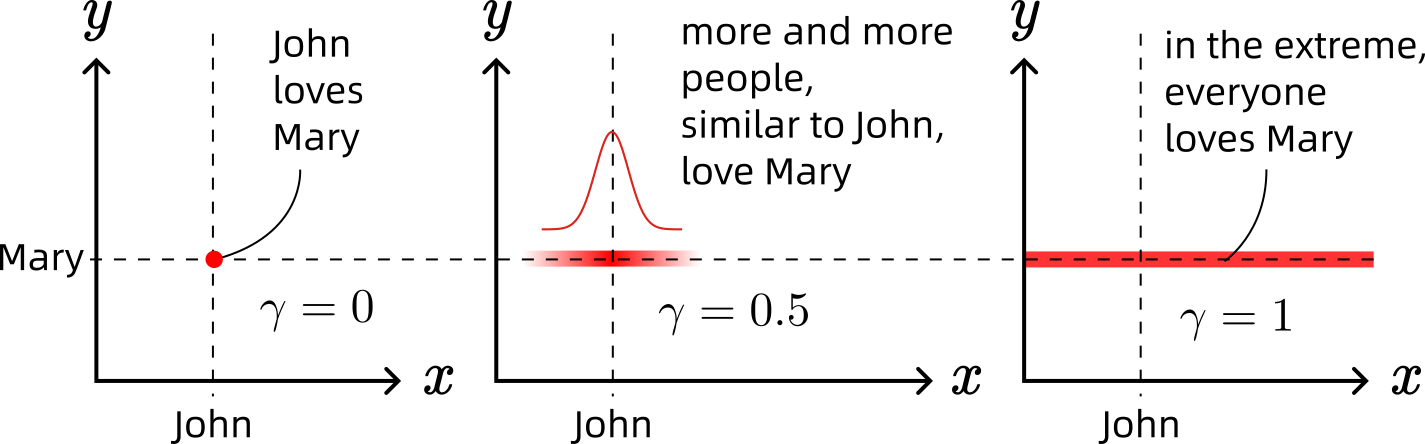
\includegraphics[scale=0.7]{cylindrify-example.png}}}
\end{equation}
The Subject Space $X$ is 1-dimensional here.  The relation $\logic{love}$ lives in $X \times X$.

\section{Variables}

The treatment of variables and their bindings is another tricky problem.  Our solution follows Paul Halmos' approach developed in the 1950s \cite{Halmos1962}.  In his \textbf{monadic logic}, where predicates are functions $P: X \rightarrow \Omega$, there could only be one variable living in the Subject Space $X$.  In his \textbf{polyadic logic}, predicates can take on more than one arguments, which involves multiple copies of the Subject Space $X$.  He constructs $X^I$ where $I$ is an index set of ``variables,'' even though they themselves don't really change.  For example, $I = \{1,2,3,4\}$ provides 4 variable ``slots''.

The implementation can be illustrated as follows:
\begin{align}
\nonumber
& \qquad \qquad \tikzmark{Slot1}
\setlength{\fboxrule}{3pt}
\fcolorbox{cyan!70}{white}{$\mbox{slot}_1$}
\qquad
\tikzmark{Slot2} \fcolorbox{cyan!70}{white}{$\mbox{slot}_2$}
\qquad
\tikzmark{Slot3} \fcolorbox{cyan!70}{white}{$\mbox{slot}_3$} \\
& \quad \mbox{weights} \\
& \nonumber \\
& \logic{father}(\tikzmark{x11} x_{11}, \tikzmark{x12} x_{12}, \tikzmark{x13} -_{13}) \wedge
\logic{father}(\tikzmark{x21} -_{21}, \tikzmark{x22} x_{22}, \tikzmark{x23} x_{23}) \rightarrow \logic{grand\hbox{-}father}(x_1,-_2,x_3)
\nonumber
\begin{tikzpicture}[remember picture,overlay]
\draw (pic cs:Slot1) +(20pt,-7pt) -- ($ (pic cs:x11) +(7pt,12pt) $);
\draw (pic cs:Slot1) +(20pt,-7pt) -- ($ (pic cs:x12) +(7pt,12pt) $);
\draw (pic cs:Slot1) +(20pt,-7pt) -- ($ (pic cs:x13) +(7pt,12pt) $);
\draw (pic cs:Slot1) +(20pt,-7pt) -- ($ (pic cs:x21) +(7pt,12pt) $);
\draw (pic cs:Slot1) +(20pt,-7pt) -- ($ (pic cs:x22) +(7pt,12pt) $);
\draw (pic cs:Slot1) +(20pt,-7pt) -- ($ (pic cs:x23) +(7pt,12pt) $);
\draw (pic cs:Slot2) +(20pt,-7pt) -- ($ (pic cs:x11) +(7pt,12pt) $);
\draw (pic cs:Slot2) +(20pt,-7pt) -- ($ (pic cs:x12) +(7pt,12pt) $);
\draw (pic cs:Slot2) +(20pt,-7pt) -- ($ (pic cs:x13) +(7pt,12pt) $);
\draw (pic cs:Slot2) +(20pt,-7pt) -- ($ (pic cs:x21) +(7pt,12pt) $);
\draw (pic cs:Slot2) +(20pt,-7pt) -- ($ (pic cs:x22) +(7pt,12pt) $);
\draw (pic cs:Slot2) +(20pt,-7pt) -- ($ (pic cs:x23) +(7pt,12pt) $);
\draw (pic cs:Slot3) +(20pt,-7pt) -- ($ (pic cs:x11) +(7pt,12pt) $);
\draw (pic cs:Slot3) +(20pt,-7pt) -- ($ (pic cs:x12) +(7pt,12pt) $);
\draw (pic cs:Slot3) +(20pt,-7pt) -- ($ (pic cs:x13) +(7pt,12pt) $);
\draw (pic cs:Slot3) +(20pt,-7pt) -- ($ (pic cs:x21) +(7pt,12pt) $);
\draw (pic cs:Slot3) +(20pt,-7pt) -- ($ (pic cs:x22) +(7pt,12pt) $);
\draw (pic cs:Slot3) +(20pt,-7pt) -- ($ (pic cs:x23) +(7pt,12pt) $);
\end{tikzpicture}
\end{align}
Every argument in the lower row has the potential to end up in any slot on the upper row.  For each slot, we take a \textbf{Softmax} to ``select'' one argument as the ``winner''.  Such parallel application of Softmax has essentially the same structure as -- surprise? -- \textbf{Self Attention}.

The rest of my thesis will explain these constructions in more details, but once the reader understands the principles behind them, the tedious details kind of fall into place naturally.